\section{For the below figure}
    \begin{figure}[H]
        \centering
        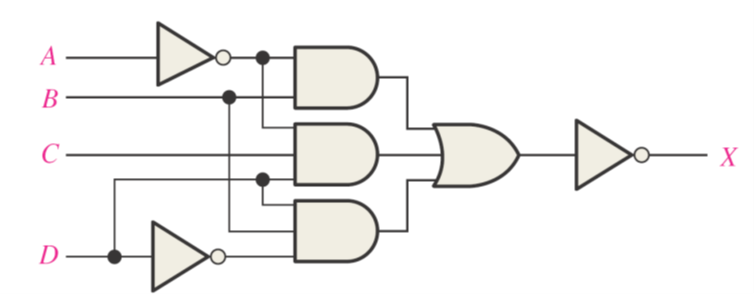
\includegraphics[width=0.5\textwidth]{pictures/1_diagram.png}
        \caption{Sơ đồ mạch bài 1}
    \end{figure}
    \subsection{Derive the output and minimize the output function using Karnaugh map}
        \hspace*{0.6cm}Từ sơ đồ mạch ta có giá trị đầu ra:
        \begin{align*}
            X(A, B, C, D) &= \overline{(\bar{A} \cdot B) + (\bar{A} \cdot C \cdot D) + (B \cdot D \cdot \bar{D})} \\
            &= \overline{(\bar{A} \cdot B) + (\bar{A} \cdot C \cdot D)}  
        \end{align*}
        \hspace*{0.6cm}Rút gọn biểu thức bằng bìa Karnaugh:
        \begin{align*}
            X(A, B, C, D) &= \overline{(01)(01 + 10 + 01 + 00) + 0(0 + 1) (11)} \\
            &= \overline{0111 + 0110 + 0101 + 0100 + 0011 + 0111} \\
            &= \overline{\sum{(7,6,5,4,3)}} = \sum{(0,1,2,8,9,10,11,12,13,14,15)} \\
        \end{align*}
        \hspace*{0.6cm}Vậy ta có bảng Karnaugh và biểu thức rút gọn:
        \begin{figure}[H]
            \centering
            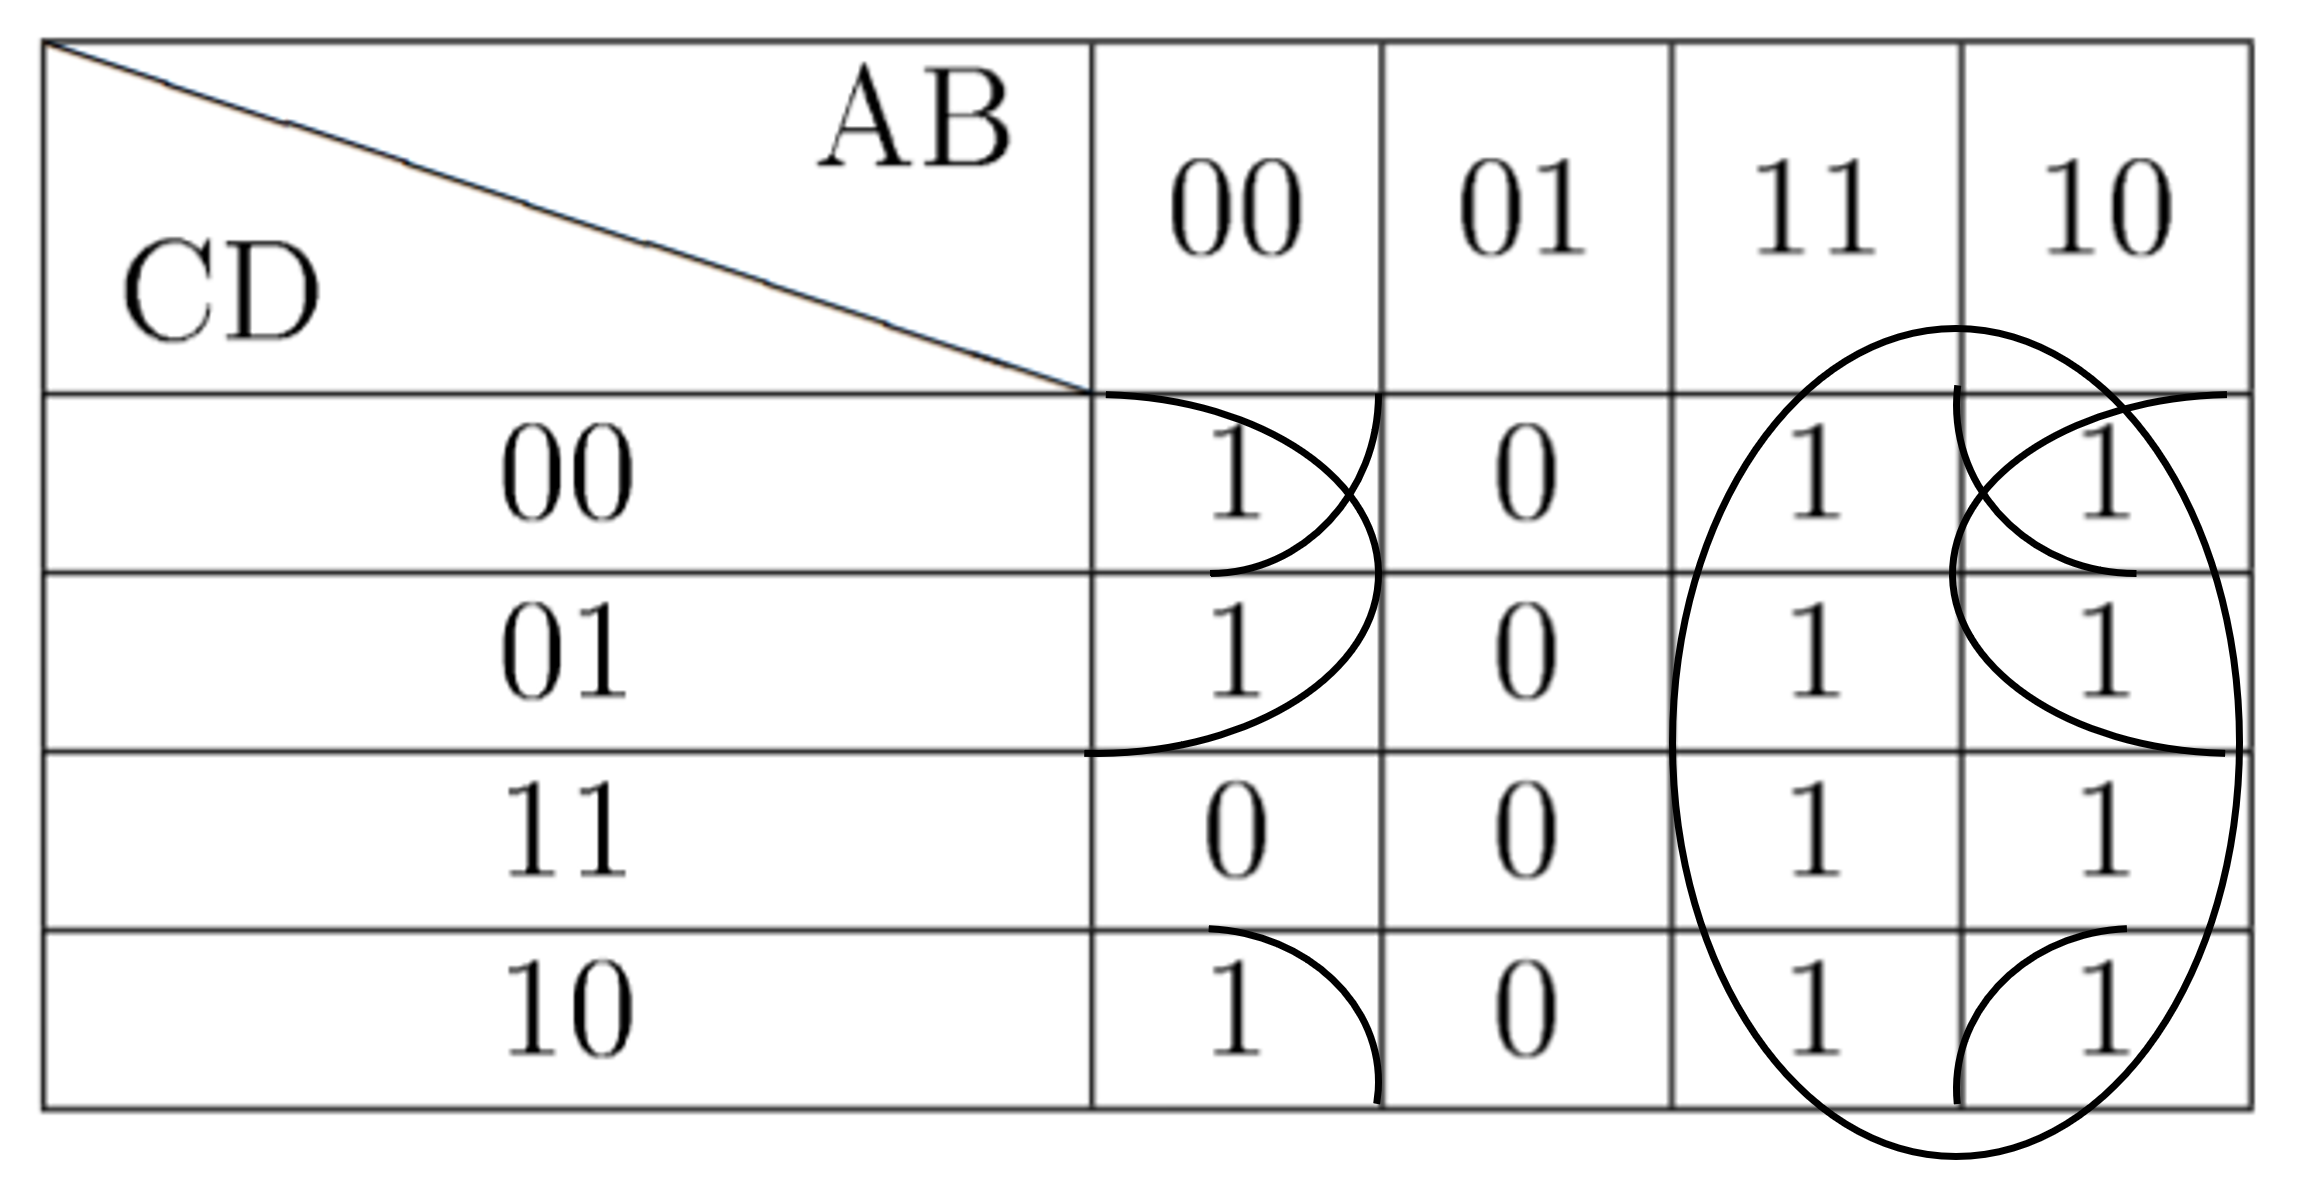
\includegraphics[width=0.5\textwidth]{pictures/1_karnaugh.png}
            \caption{Bảng Karnaugh bài 1}
        \end{figure}
        Từ bảng Karnaugh ta có biểu thức rút gọn:
        \begin{align*}
            X(A, B, C, D) &= \sum{(0,1,2,8,9,10,11,12,13,14,15)} = \bar{B}\bar{C} + \bar{B}\bar{D} + A\\
        \end{align*}
    \subsection{Draw the wave form of output if}
        \begin{figure}[H]
            \centering
            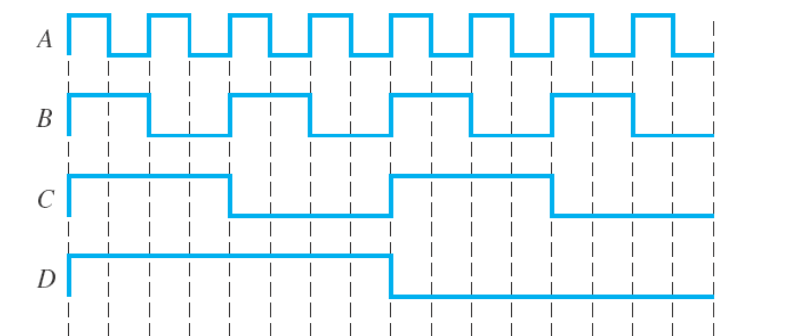
\includegraphics[width=0.8\textwidth]{pictures/1_waveinput.png}
            \caption{Waveform input bài 1}
            \label{fig:1_waveinput}
        \end{figure}
        \hspace*{0.6cm}Từ biểu thức rút gọn và đầu vào như hình \ref{fig:1_waveinput} ta có đầu ra như hình \ref{fig:1_waveoutput}
        \begin{figure}[H]
            \centering
            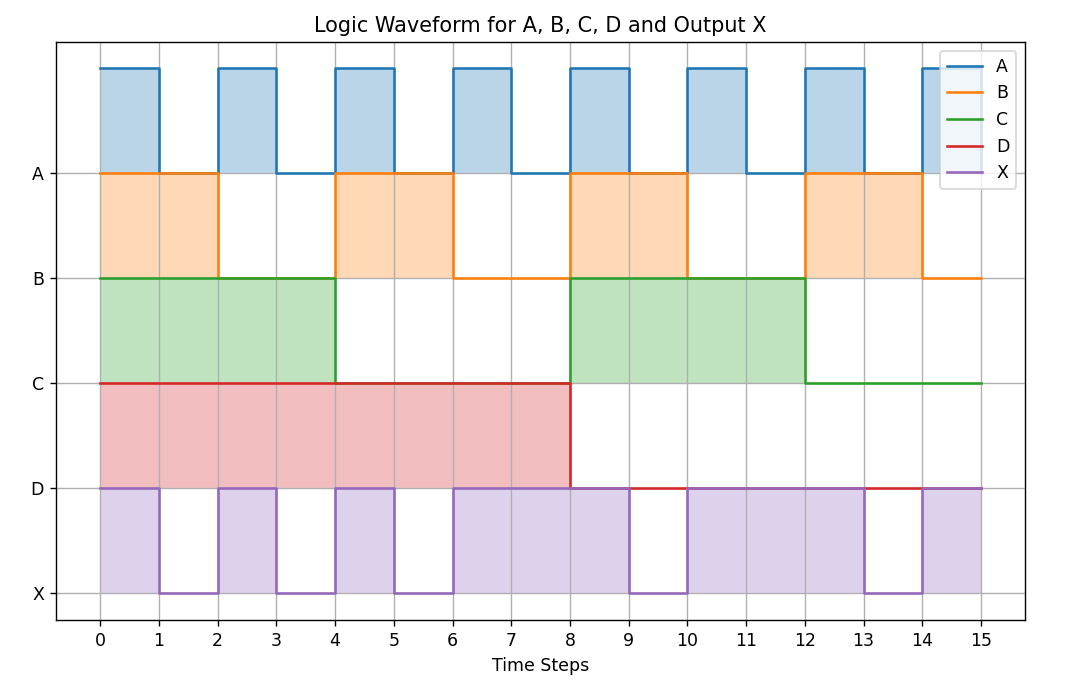
\includegraphics[width=0.8\textwidth]{pictures/1_waveoutput.png}
            \caption{Waveform output bài 1}
            \label{fig:1_waveoutput}
        \end{figure}
        